\section{Problem Statement}
The German parliament, called the \emph{Bundestag}, publishes the proceedings of
their meetings, as an effort to open up the political process to the common
people. These proceedings have been continously published starting in 1949.
Figure~\ref{fig:pdf_page} shows a sample page from one of these proceedings; the
left column contains a continuation of a speech from the previous page as well
as two moderately sized speeches, while the right column contains a large number
of very short speeches. Having a large corpus of political proceedings like this
is wonderful and opens a lot of doors for research regarding political
discourse. Figure~\ref{fig:pdf_roi} shows the same page seen in
Figure~\ref{fig:pdf_page}, but with a number of regions of interest (manually)
colored in. Unfortunately this data is only available as PDF files, which in
terms of internal representation are entirely unstructured. That means that none
of the rich structure highlighted in Figure~\ref{fig:pdf_roi} is actually
present in a computer-usable way.

\begin{figure}[htbp]
  \centering
  \includegraphics[page=16,height=0.95\textheight]{../pdfs/18001.pdf}
  \caption{A sample page from one of the Bundestag proceedings.}
  \label{fig:pdf_page}
\end{figure}
\begin{figure}[htbp]
  \centering
  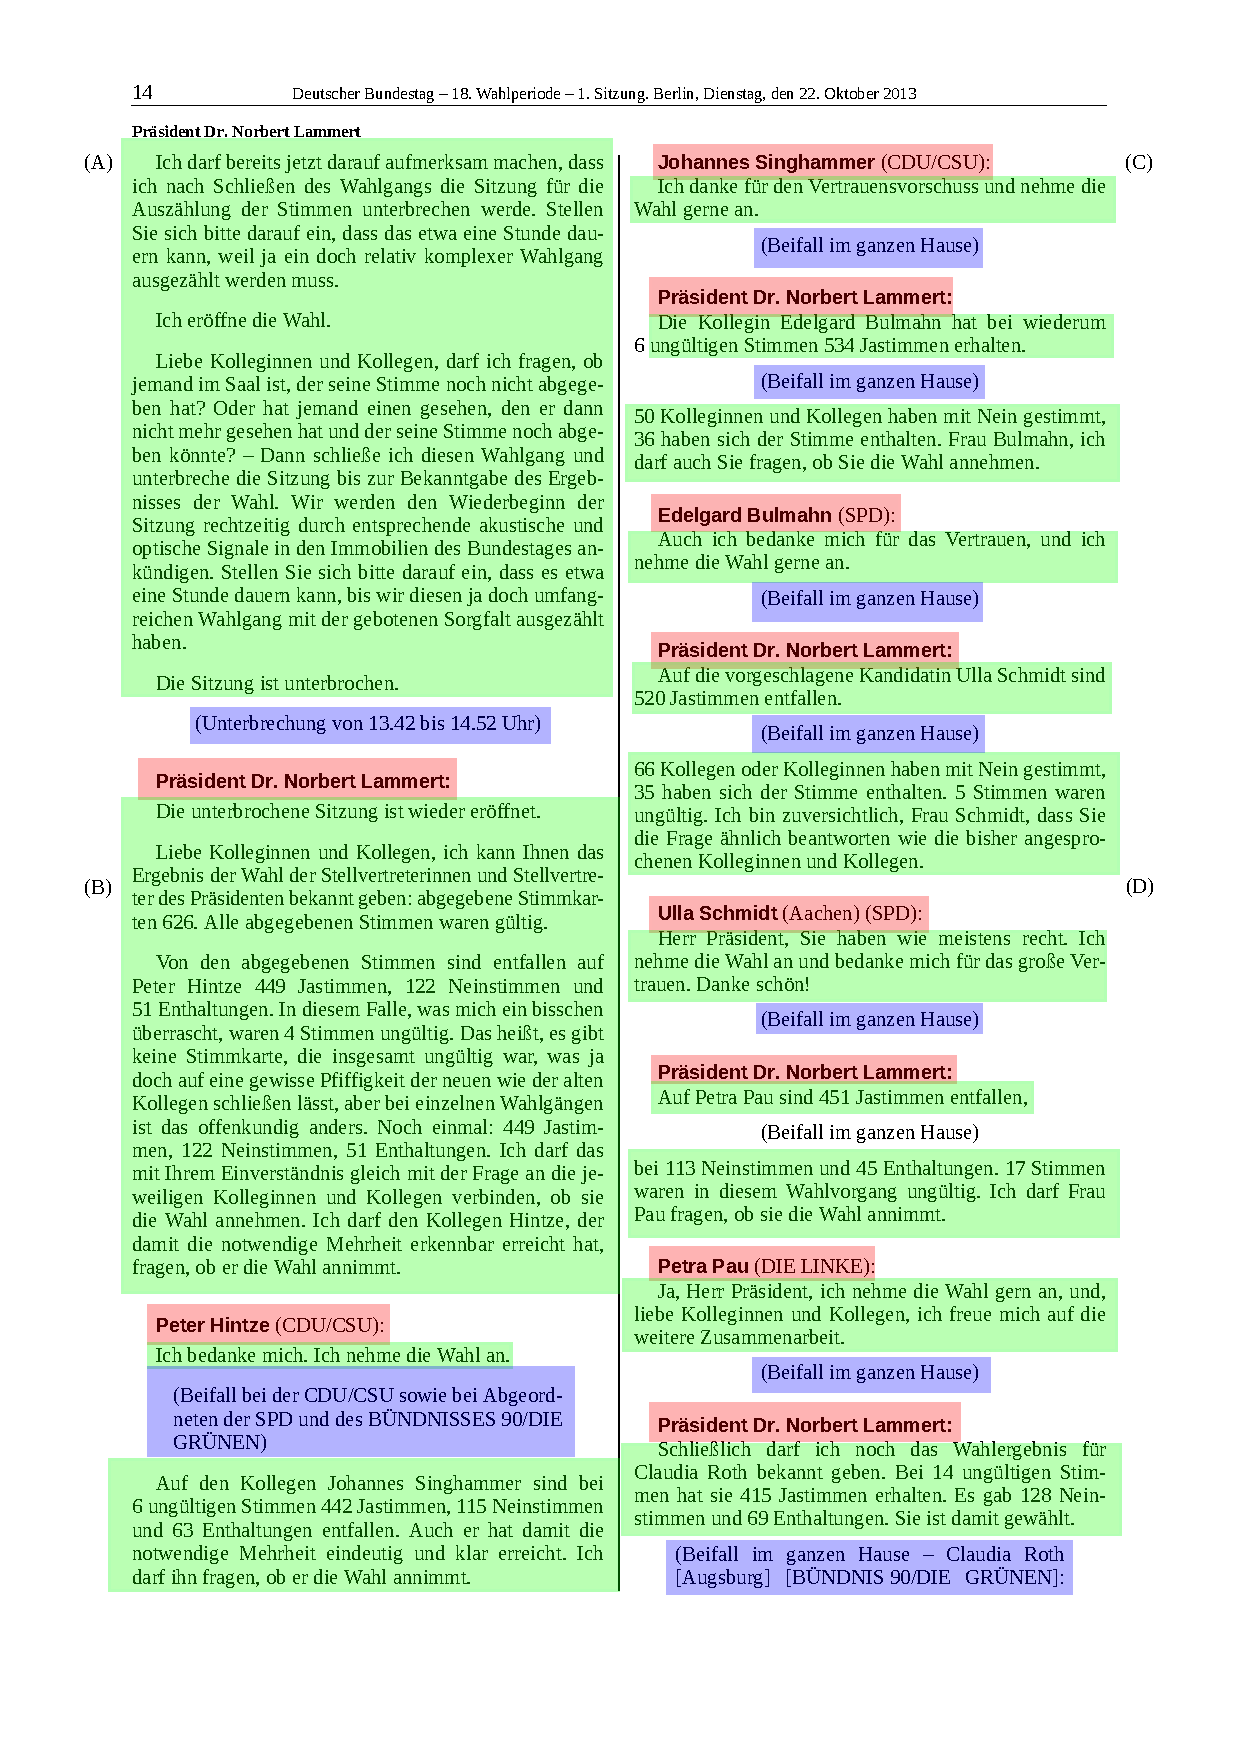
\includegraphics[height=0.85\textheight]{figures/pdf_roi.pdf}
  \caption{The same page as in Figure~\ref{fig:pdf_page}, hand-annotated with
    interesting regions that play a significant role in understanding the
    layout. The red regions are the headers the signify that someone is starting
    a speech, and contain information about who the speakers is. The blue
    regions are little interruptions (\emph{Heiterkeits}), often signifying
    approval or displeasure (the regularly seen \emph{Beifall} means applause).
    The green regions indicate plain blocks of text.}
  \label{fig:pdf_roi}
\end{figure}

The central problem in this thesis is the extraction of speeches from the
documents, transforming each document into a structured series of speeches that
can be serve as a useful entry point into further research. As a first step, the
structural layout (as in Figure~\ref{fig:pdf_roi}) will be extracted using
unsupervised clustering algorithms. The textual contents of the document are
then fed into supervised text classifier, where each piece of text is augmented
with the corresponding layout information previously obtained. More details on
this process will be supplied in Section~\ref{sec:method}.

As annotating data by hand is an expensive process, a big focus is on limiting
the amount of required training data as much as possible; it would be preferable
if the system was able to learn sufficiently from a handful (say, less than 5)
of hand-annotated files.

\subsection{Dataset}
PDF files are unfortunately rather difficult to work with; being a vector-based
format, they have no internal concept of words or sentences. All that's
available are instructions for drawing a certain character at a certain
position. This means that even something as seemingly trivial as obtaining the
lines of text from a PDF requires some fairly involved logic and heuristics (for
instance, one would think that simply taking all characters on a page with the
same $y$ coordinate would be sufficient until realizing that many documents have
a layout with two columns of text). This is dealt with by using the
\texttt{pdftohtml} script from the Poppler PDF rendering
library\footnote{https://poppler.freedesktop.org/}. This script converts a PDF
file to an XML file containing logical lines of text along with the coordinates
and size of the line. Figure~\ref{fig:example} shows an example of a portion of
a PDF file and the corresponding XML. The contents of the \texttt{text} elements
forms the plaintext that is fed into the classification algorithm. Although the
layout information contained in the properties (\texttt{top}, \texttt{left},
\texttt{width}, \texttt{height} and \texttt{font}) could be used for the layout
clustering, this would effectively tie the performance of the clustering to the
performance of \texttt{pdftohtml}'s line-extraction heuristics. Instead, a
separate system is used (the Apache pdfbox\footnote{https://pdfbox.apache.org/}
library for Java). By using the bounding boxes of individual characters as the
base for clustering, the troubles of line-extraction can be fully bypassed.

\begin{figure}[htbp]
  \centering
  \begin{subfigure}[b]{0.6\textwidth} 
    \centering
    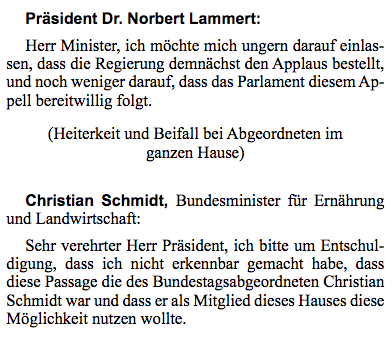
\includegraphics[width=\textwidth]{figures/source.png}
    \caption{A portion of the source PDF.}
    \label{fig:source_pdf}
  \end{subfigure}
  \begin{subfigure}[b]{\textwidth}
	\centering
    \begin{lstlisting}[language=xml, morekeywords={text}]
      <text top="122" left="125" width="143" height="16" font="3">
          <b>Dr. Norbert Lammert </b>
      </text>
      <text top="122" left="269" width="83" height="17" font="4">
          (CDU/CSU):
      </text>
      <text top="142" left="125" width="328" height="17" font="4">
          Herr Alterspräsident, lieber Kollege Riesenhuber, ich
      </text>
      <text top="158" left="108" width="156" height="17" font="4">
          nehme die Wahl gerne an.
      </text>
      <text top="186" left="141" width="278" height="17" font="4">
          (Beifall im ganzen Hause – Abgeordnete aller
      </text>
      <text top="203" left="158" width="242" height="17" font="4">
          Fraktionen gratulieren dem Präsidenten)
      </text>
    \end{lstlisting}
    \caption{XML created by running \texttt{pdftohtml}, corresponding to the PDF
      excerpt in Figure~\ref{fig:source_pdf}. The contents of the \texttt{text}
      elements are used as inputs for the classification algorithm; the layout
      data contained in the properties is not used, as a separate software
      pipeline is used for the unsupervised clustering.}
    \label{fig:source_xml}
  \end{subfigure}
  \caption{A sample excerpt from a source PDF, along with its XML representation
    created by \texttt{pdftohtml}.}
  \label{fig:example}
\end{figure}

The dataset was obtained through a rule-based system as described in the
introduction, which annotates each \texttt{<text>} element of the XML files with
a boolean flag indicating whether said element starts a new speech. The system
was run on documents from the 18th electoral period of the \emph{Bundestag},
consisting of 211 documents dating from 2013 to 2017. Together these documents
contain 43,252 \texttt{<text>} elements indicating the start of speeches (that
is, positive training samples), and 2,602,793 other elements (negative samples).
This adds to a total of 2,646,045 training samples, taking up 503 MiB. This is a
rather lopsided distribution (there are roughly 60 negative samples for each
positive sample), which will have to be accounted for by, for instance, using
stratified sampling. Figure~\ref{fig:data_dist} shows the distribution of the
number of positive samples per file, giving a guideline as to how many files
would have to be annotated to reach a desired amount of positive samples.

\begin{figure}[htbp]
  \centering
  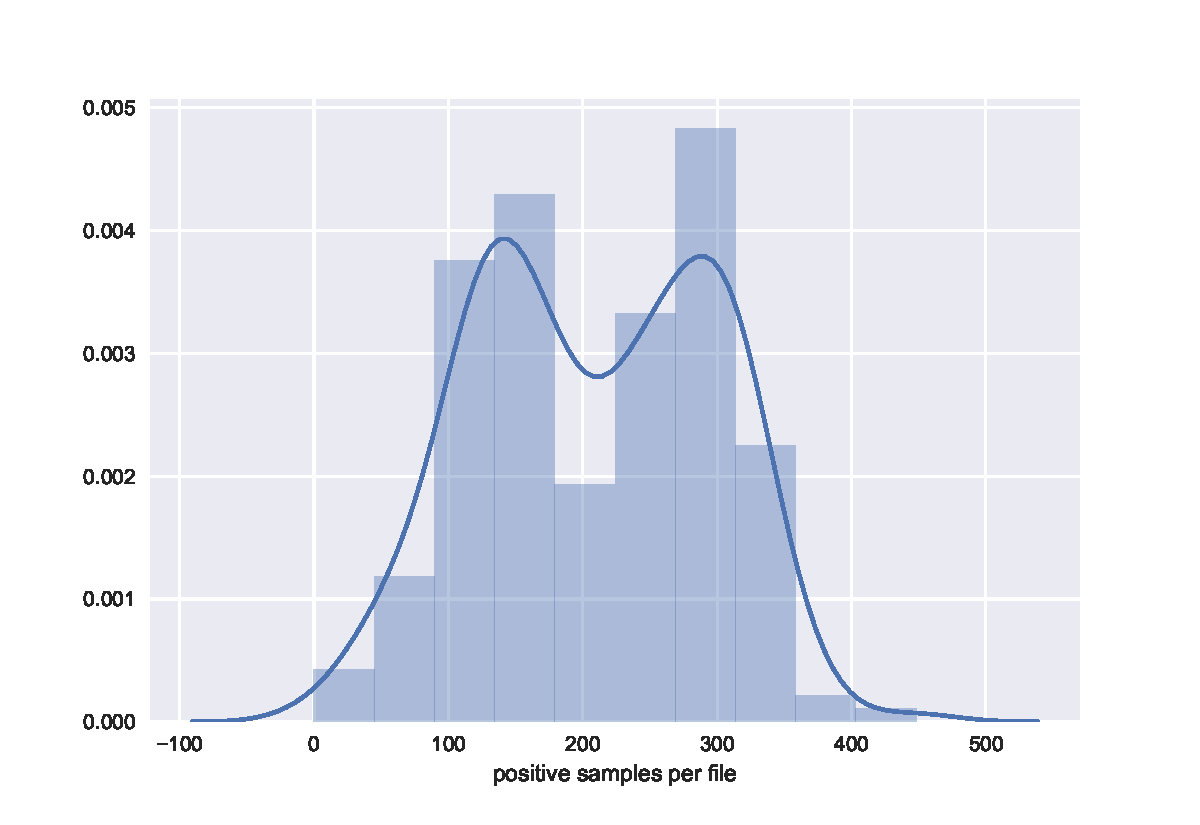
\includegraphics[width=\textwidth]{figures/distribution.pdf}
  \caption{Distribution of the number of positive samples per file}
  \label{fig:data_dist}
\end{figure}

\subsection{Research Question}
As the application of supervised text classification is fairly basic and
well-studied, academically speaking the interesting portion of this problem is
figuring out what benefit is added by the unsupervised layout clustering, if
any. A potential benefit could manifest itself in a couple of different ways:
\begin{itemize}
\item The performance (using a metric such as the F1 score or average
  precision, to be further elaborated on in Section~\ref{sec:method}) after
  training is increased.
\item The peak performance is equal, but less training data is required to reach
  said peak.
\item The peak performance is equal and a similar amount of training data is
  required, but the classifier needs less iterations to reach this performance.
\end{itemize}
This leads to the research question that is central to this thesis:
\begin{researchquestion}
  Does augmenting a text classification system with layout information obtained
  by unsupervised clustering of the input data improve the classifier with
  regards to:
  \begin{itemize}
  \item F1 score and average precision
  \item required volume of training data
  \item training speed
  \end{itemize}
\end{researchquestion}

%%% Local Variables:
%%% mode: latex
%%% TeX-master: "report"
%%% End: